\section{Introduction to Machine Learning}
    Machine learning is a subset of artificial intelligence that focuses on developing algorithms and statistical models that enable computers to learn from and make predictions based on data. 
    It is used in a wide range of applications, including image and speech recognition, medical diagnosis, and financial forecasting. 
    Machine learning can be broadly categorized into three types: supervised learning, unsupervised learning, and reinforcement learning.

    Machine learning is useful for tasks where it is difficult to explicitly program the rules or patterns, such as recognizing handwritten digits or detecting spam emails.

    By training a model on a dataset, the model can learn the underlying patterns and relationships in the data and make predictions on new, unseen data.

\section{Structure of Neural Networks}
    Neural networks are a class of machine learning models inspired by the structure and function of the human brain. They consist of interconnected nodes, or neurons, organized in layers. Each neuron receives input, processes it, and produces an output that is passed to the next layer. The connections between neurons are represented by weights, which are learned during the training process.

    \vspace{1em} \noindent The basic building block of a neural network is the perceptron, which takes a set of inputs, applies weights to them, and passes the weighted sum through an activation function to produce an output. Multiple perceptrons are connected in layers to form a neural network. The most common type of neural network is the feedforward neural network, where information flows in one direction from the input layer to the output layer.

    \vspace{1em} \noindent Neural networks can have multiple layers, with each layer performing a different transformation on the input data. The input layer receives the input data, the hidden layers process the data, and the output layer produces the final output. The number of layers and the number of neurons in each layer are hyperparameters that can be tuned to optimize the performance of the network.

    \begin{figure}[h]
        \centering
        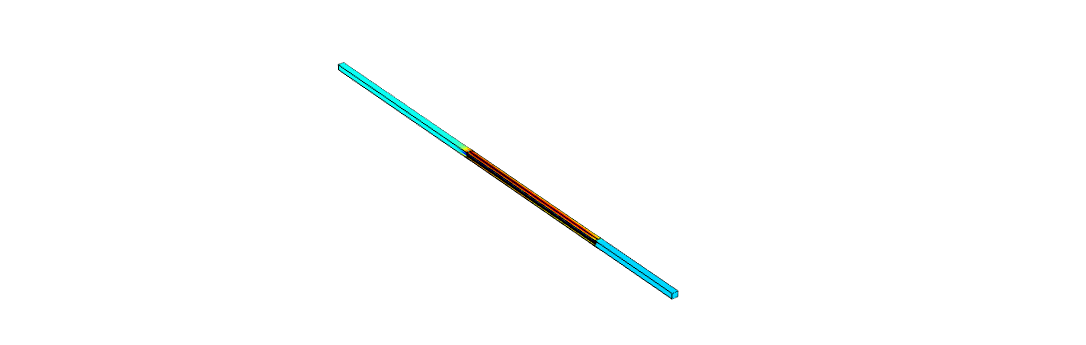
\includegraphics[width=0.8\textwidth]{00_Images/00_Velocity.png}
        \caption{Structure of a feedforward neural network.}
        \label{fig:neural_network}
    \end{figure}

    \subsection{Types of Layers}
        \noindent Neural networks have multiple types of layers, including:
            \begin{itemize}
                \item Input Layer: The first layer of the network that receives the input data.
                \item Hidden Layers: Intermediate layers that process the input data and extract features.
                \item Output Layer: The final layer that produces the output of the network.
            \end{itemize}
        \subsection{Shallow and Deep Neural Networks}
            \noindent Neural networks can be classified as shallow or deep based on the number of hidden layers they contain. Shallow networks have a small number of hidden layers, while deep networks have many hidden layers. Deep neural networks are capable of learning complex patterns and representations in the data but are more computationally intensive to train

\section{Process of Supervised Learning}
    Supervised learning is a type of machine learning where the model is trained on labeled data. The objective is to learn a function that maps input data to the correct output based on the provided labels. The general process involves the following steps:

    \begin{enumerate}
        \item \textbf{Data Collection}: Gather a dataset consisting of input-output pairs. Let \( \mathbf{X} = \{ \mathbf{x}_1, \mathbf{x}_2, \ldots, \mathbf{x}_n \} \) be the set of input vectors and \( \mathbf{Y} = \{ y_1, y_2, \ldots, y_n \} \) be the corresponding set of output values.
        
        \item \textbf{Data Preprocessing}: Clean and preprocess the data to remove noise, handle missing values, and normalize the features. This step ensures that the data is in a suitable format for training the model.
        
        \item \textbf{Model Selection}: Choose a neural network architecture suitable for the problem. This includes deciding on the number of layers, the number of neurons per layer, and the type of activation functions.
        
        \item \textbf{Initialization}: Initialize the weights \( \mathbf{W} \) and biases \( \mathbf{b} \) of the network. This is typically done using small random values.
        
        \item \textbf{Forward Propagation}: Compute the predicted output \( \hat{y} \) by passing the input \( \mathbf{x} \) through the network.
        
        \item \textbf{Loss Computation}: Calculate the loss \( \mathcal{L}(\hat{y}, y) \) which measures the difference between the predicted output \( \hat{y} \) and the actual output \( y \).
        
        \item \textbf{Backward Propagation}: Compute the gradients of the loss with respect to the weights and biases.
        
        \item \textbf{Weight Update}: Update the weights and biases using an optimization algorithm such as Stochastic Gradient Descent (SGD).
        
        \item \textbf{Model Evaluation}: Evaluate the performance of the model on a validation set to tune hyperparameters and avoid overfitting.
    \end{enumerate}

    \noindent Mathematically, the process can be summarized as follows:

    \vspace{1em} \noindent Given an input vector \( \mathbf{x} \), the network's output \( \hat{y} \) is computed as:
    \begin{equation}
    \hat{y} = f(\mathbf{x}; \mathbf{W}, \mathbf{b})
    \end{equation}

    \noindent where \( f \) is the function represented by the neural network, parameterized by weights \( \mathbf{W} \) and biases \( \mathbf{b} \).

    \vspace{1em} \noindent The loss function \( \mathcal{L} \) is defined to measure the discrepancy between \( \hat{y} \) and the true output \( y \):
    \begin{equation}
    \mathcal{L}(\hat{y}, y)
    \end{equation}

    \vspace{1em} \noindent The gradients of the loss with respect to the parameters are computed during backpropagation:
    \begin{equation}
    \frac{\partial \mathcal{L}}{\partial \mathbf{W}}, \quad \frac{\partial \mathcal{L}}{\partial \mathbf{b}}
    \end{equation}

    \noindent Finally, the parameters are updated using an optimization algorithm:
    \begin{equation}
    \mathbf{W} \leftarrow \mathbf{W} - \eta \frac{\partial \mathcal{L}}{\partial \mathbf{W}}, \quad \mathbf{b} \leftarrow \mathbf{b} - \eta \frac{\partial \mathcal{L}}{\partial \mathbf{b}}
    \end{equation}

    \noindent where \( \eta \) is the learning rate.

    \begin{figure}[h]
    \centering
    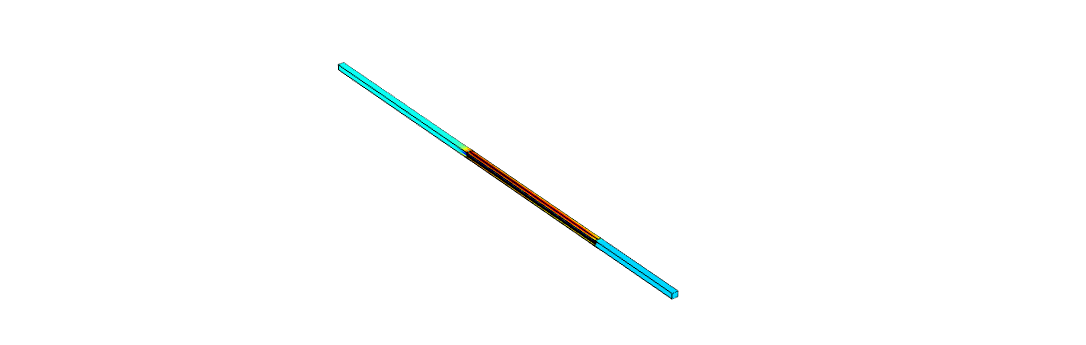
\includegraphics[width=0.8\textwidth]{00_Images/00_Velocity.png}
    \caption{Overview of the supervised learning process in neural networks.}
    \label{fig:supervised_learning}
    \end{figure}

\section{Forward Propogation}
    Forward propagation is the process by which the input is passed through the neural network to obtain the output. It involves the computation of outputs at each layer of the network until the final output is achieved. The process can be described as follows:

    Given an input vector \( \mathbf{x} \), the output of the first layer is computed as:
    \begin{equation}
    \mathbf{z}^{(1)} = \mathbf{W}^{(1)} \mathbf{x} + \mathbf{b}^{(1)}
    \end{equation}
    \begin{equation}
    \mathbf{a}^{(1)} = \sigma(\mathbf{z}^{(1)})
    \end{equation}

    where \( \mathbf{W}^{(1)} \) and \( \mathbf{b}^{(1)} \) are the weights and biases of the first layer, \( \mathbf{z}^{(1)} \) is the linear combination of inputs and weights, and \( \sigma \) is the activation function.

    This process is repeated for each subsequent layer. For the \( l \)-th layer, the computations are:
    \begin{equation}
    \mathbf{z}^{(l)} = \mathbf{W}^{(l)} \mathbf{a}^{(l-1)} + \mathbf{b}^{(l)}
    \end{equation}
    \begin{equation}
    \mathbf{a}^{(l)} = \sigma(\mathbf{z}^{(l)})
    \end{equation}

    Finally, the output of the network is obtained:
    \begin{equation}
    \hat{y} = \mathbf{a}^{(L)}
    \end{equation}

    where \( L \) is the number of layers in the network.

    \begin{figure}[h]
        \centering
        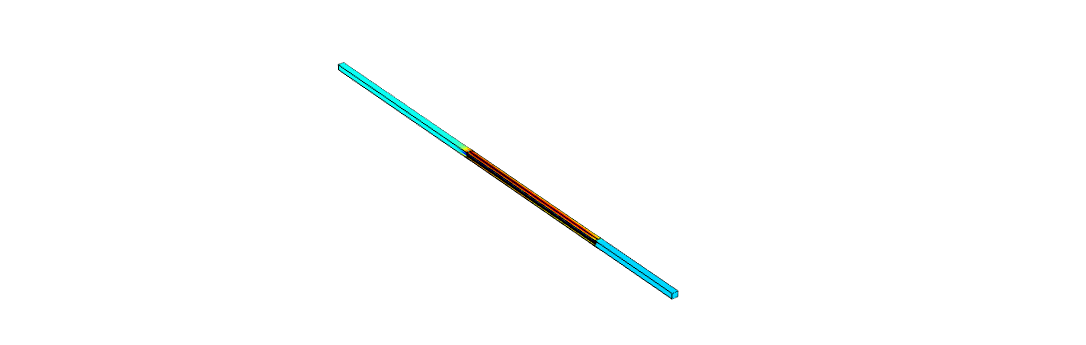
\includegraphics[width=0.8\textwidth]{00_Images/00_Velocity.png}
        \caption{Forward propagation through a neural network.}
        \label{fig:forward_propagation}
    \end{figure}

        \subsection{Activation Functions}

            Activation functions introduce non-linearity into the neural network, allowing it to learn complex patterns. Common activation functions include:

            \subsubsection{Sigmoid}

                The sigmoid function is defined as:
                \begin{equation}
                \sigma(z) = \frac{1}{1 + e^{-z}}
                \end{equation}
                It maps any real-valued number into the range (0, 1).

            \subsubsection{Hyperbolic Tangent (Tanh)}

                The tanh function is defined as:
                \begin{equation}
                \sigma(z) = \tanh(z) = \frac{e^z - e^{-z}}{e^z + e^{-z}}
                \end{equation}
                It maps any real-valued number into the range (-1, 1).

            \subsubsection{Rectified Linear Unit (ReLU)}

                The ReLU function is defined as:
                \begin{equation}
                \sigma(z) = \max(0, z)
                \end{equation}
                It outputs the input directly if it is positive; otherwise, it outputs zero.

            \subsubsection{Leaky ReLU}

                The Leaky ReLU function is defined as:
                \begin{equation}
                \sigma(z) = \begin{cases}
                z & \text{if } z \geq 0 \\
                \alpha z & \text{if } z < 0
                \end{cases}
                \end{equation}
                where \( \alpha \) is a small constant.

            \begin{figure}[h]
                \centering
                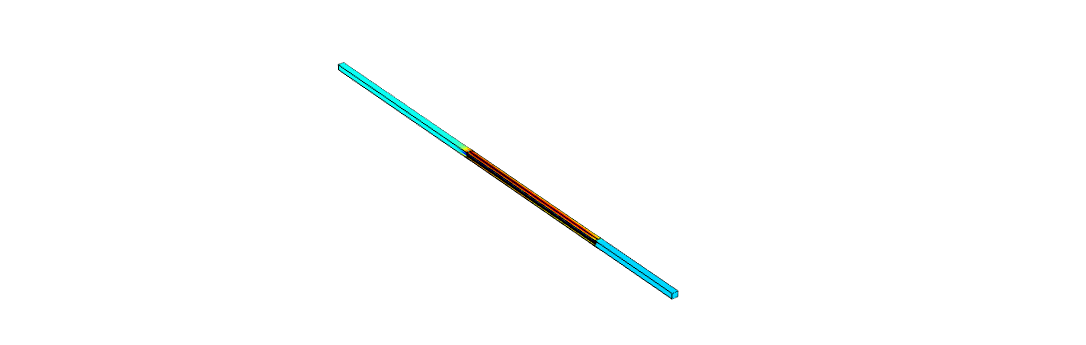
\includegraphics[width=0.8\textwidth]{00_Images/00_Velocity.png}
                \caption{Common activation functions used in neural networks.}
                \label{fig:activation_functions}
            \end{figure}

\section{Backward Propagation}

    Backward propagation, or backpropagation, is the process by which neural networks update their weights and biases to minimize the loss function. It involves calculating the gradient of the loss function with respect to each weight by the chain rule, iterating backward from the output layer to the input layer. The main steps are as follows:
    
    \begin{enumerate}
        \item \textbf{Compute the loss}: Calculate the loss \( \mathcal{L} \) between the predicted output \( \hat{y} \) and the actual output \( y \).
        \item \textbf{Calculate the gradient of the loss with respect to the output layer}: For the output layer, compute the gradient of the loss with respect to the activations.
        \item \textbf{Propagate the gradient backward through the network}: Use the chain rule to compute the gradient of the loss with respect to the weights and biases of each layer.
        \item \textbf{Update the weights and biases}: Use the gradients to update the weights and biases in a direction that reduces the loss.
    \end{enumerate}
    
    Mathematically, the gradient of the loss \( \mathcal{L} \) with respect to the weights \( \mathbf{W}^{(l)} \) and biases \( \mathbf{b}^{(l)} \) in layer \( l \) is computed as:
    
    \begin{equation}
    \frac{\partial \mathcal{L}}{\partial \mathbf{W}^{(l)}} = \delta^{(l)} \mathbf{a}^{(l-1)} 
    \end{equation}
    
    \begin{equation}
    \frac{\partial \mathcal{L}}{\partial \mathbf{b}^{(l)}} = \delta^{(l)}
    \end{equation}
    
    where \( \delta^{(l)} \) is the error term for layer \( l \) and \( \mathbf{a}^{(l-1)} \) is the activation of the previous layer.
    
    The error term \( \delta^{(l)} \) is computed as:
    
    \begin{equation}
    \delta^{(l)} = \begin{cases} 
    (\mathbf{a}^{(L)} - y) \odot \sigma'(\mathbf{z}^{(L)}) & \text{for the output layer} \\
    (\mathbf{W}^{(l+1)})^T \delta^{(l+1)} \odot \sigma'(\mathbf{z}^{(l)}) & \text{for hidden layers}
    \end{cases}
    \end{equation}
    
    where \( \odot \) denotes the element-wise multiplication and \( \sigma' \) is the derivative of the activation function.
    
    \subsection{Loss Functions}
    
        Loss functions, also known as cost functions, measure how well the neural network's predictions match the actual target values. Common loss functions include:
    
        \subsubsection{Mean Squared Error (MSE)}
    
            The Mean Squared Error is used for regression tasks and is defined as:
    
            \begin{equation}
            \mathcal{L}_{\text{MSE}} = \frac{1}{n} \sum_{i=1}^n (\hat{y}_i - y_i)^2
            \end{equation}
            
            \begin{figure}[h]
                \centering
                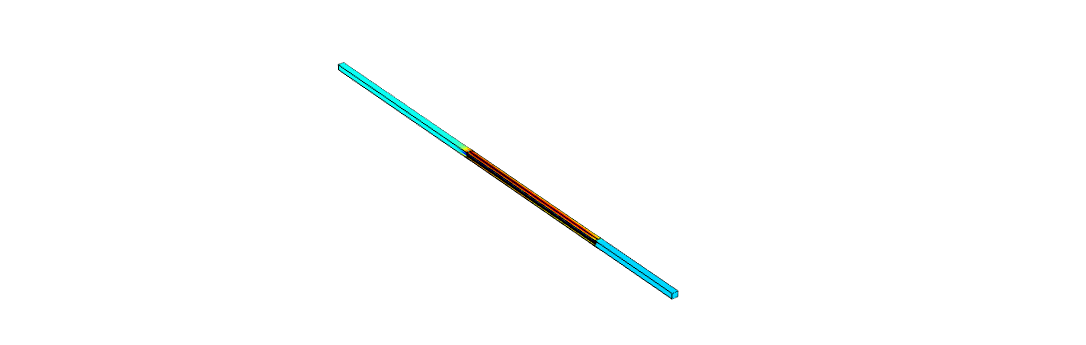
\includegraphics[width=0.8\textwidth]{00_Images/00_Velocity.png}
                \caption{Illustration of common loss functions.}
                \label{fig:loss_functions}
            \end{figure}
    
    \subsection{Methods to Update Weights}
    
        Updating the weights and biases of a neural network is a crucial part of the training process. Various methods can be employed to perform these updates:
    
        \subsubsection{Stochastic Gradient Descent (SGD)}
    
            SGD updates the weights using a single training example at a time:
    
            \begin{equation}
            \mathbf{W} \leftarrow \mathbf{W} - \eta \frac{\partial \mathcal{L}}{\partial \mathbf{W}}
            \end{equation}
    
            where \( \eta \) is the learning rate.
    
        \subsubsection{Batch Gradient Descent}
    
            Batch Gradient Descent computes the gradient using the entire training dataset:
            
            \begin{equation}
            \mathbf{W} \leftarrow \mathbf{W} - \eta \frac{1}{n} \sum_{i=1}^n \frac{\partial \mathcal{L}_i}{\partial \mathbf{W}}
            \end{equation}
    
        \subsubsection{Mini-Batch Gradient Descent}
    
            Mini-Batch Gradient Descent is a compromise between SGD and Batch Gradient Descent. It uses a small random subset (mini-batch) of the training data to compute the gradient:
    
            \begin{equation}
            \mathbf{W} \leftarrow \mathbf{W} - \eta \frac{1}{m} \sum_{i=1}^m \frac{\partial \mathcal{L}_i}{\partial \mathbf{W}}
            \end{equation}
    
            where \( m \) is the mini-batch size.
    
            \subsubsection{Adaptive Methods}
    
                Adaptive methods like AdaGrad, RMSProp, and Adam adjust the learning rate based on the history of the gradients. For example, the Adam optimization algorithm updates the weights as follows:
                
                \begin{equation}
                \mathbf{m}_t = \beta_1 \mathbf{m}_{t-1} + (1 - \beta_1) \frac{\partial \mathcal{L}}{\partial \mathbf{W}}
                \end{equation}
                
                \begin{equation}
                \mathbf{v}_t = \beta_2 \mathbf{v}_{t-1} + (1 - \beta_2) \left( \frac{\partial \mathcal{L}}{\partial \mathbf{W}} \right)^2
                \end{equation}
                
                \begin{equation}
                \hat{\mathbf{m}}_t = \frac{\mathbf{m}_t}{1 - \beta_1^t}
                \end{equation}
                
                \begin{equation}
                \hat{\mathbf{v}}_t = \frac{\mathbf{v}_t}{1 - \beta_2^t}
                \end{equation}
                
                \begin{equation}
                \mathbf{W} \leftarrow \mathbf{W} - \eta \frac{\hat{\mathbf{m}}_t}{\sqrt{\hat{\mathbf{v}}_t} + \epsilon}
                \end{equation}
                
                where \( \beta_1 \) and \( \beta_2 \) are hyperparameters, \( \mathbf{m}_t \) and \( \mathbf{v}_t \) are the first and second moment estimates, and \( \epsilon \) is a small constant.
                
            \begin{figure}[h]
                \centering
                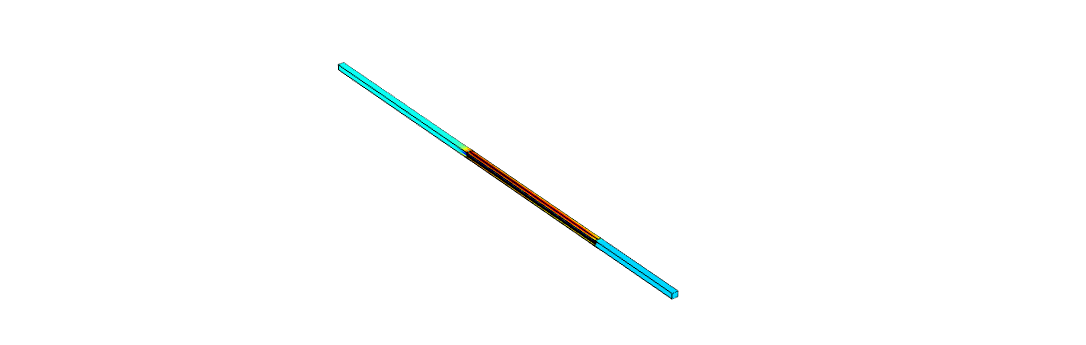
\includegraphics[width=0.8\textwidth]{00_Images/00_Velocity.png}
                \caption{Comparison of different methods to update weights.}
                \label{fig:update_methods}
            \end{figure}


\section{Hyperparameter Optimization}

    Hyperparameter optimization involves finding the optimal set of hyperparameters that result in the best performance of the neural network. Common methods for hyperparameter optimization include:

    \subsection{Grid Search}

        Grid search involves specifying a set of values for each hyperparameter and training the model on all possible combinations of these values. It is computationally expensive but exhaustive.

        \begin{equation}
        \text{Optimal Hyperparameters} = \arg \min_{\eta, \text{batch size}, \ldots} \text{Validation Loss}
        \end{equation}

    \subsection{Random Search}

        Random search samples random combinations of hyperparameters from a predefined distribution. It is often more efficient than grid search and can find good hyperparameters with fewer iterations.

        \begin{equation}
        \text{Optimal Hyperparameters} = \arg \min_{\eta, \text{batch size}, \ldots} \text{Validation Loss}
        \end{equation}

    \subsection{Bayesian Optimization}

        Bayesian optimization builds a probabilistic model of the objective function and uses it to select the most promising hyperparameters to evaluate next. It is more sophisticated and can find optimal hyperparameters more efficiently.

        \begin{equation}
        \text{Optimal Hyperparameters} = \arg \max_{\eta, \text{batch size}, \ldots} P(\text{Low Validation Loss} \mid \eta, \text{batch size}, \ldots)
        \end{equation}

    \subsection{Hyperband}

        Hyperband is a method that combines random search with early stopping. It evaluates many configurations with a small number of iterations and progressively increases the budget for the most promising configurations.

        \begin{equation}
        \text{Optimal Hyperparameters} = \arg \min_{\eta, \text{batch size}, \ldots} \text{Validation Loss}
        \end{equation}

\begin{figure}[h]
    \centering
    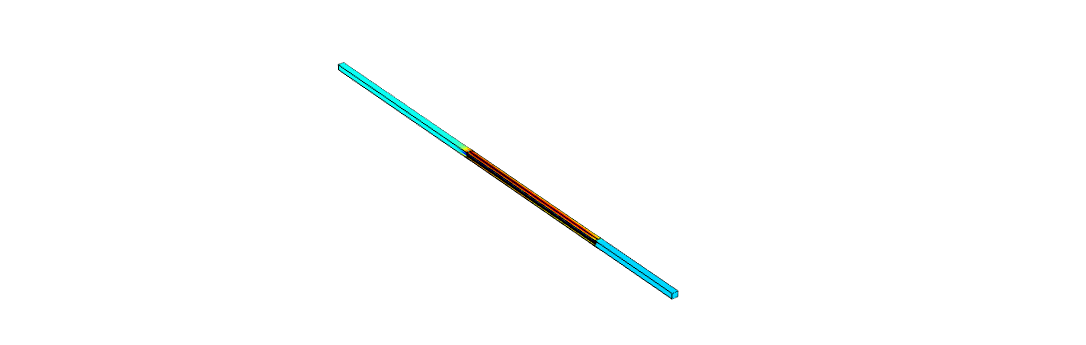
\includegraphics[width=0.8\textwidth]{00_Images/00_Velocity.png}
    \caption{Comparison of different hyperparameter optimization methods.}
    \label{fig:hyperparameter_optimization}
\end{figure}

\section{Mathematical Formulation of Neural Networks}
        \subsection{Introduction}
        This paper explores simple regression models to demonstrate the underlying mechanics by implementing these models both through MATLAB and using a paper-and-pen approach for a shallow and deep neural network.

        \newpage \subsection{Notation}
        The following table summarizes the notation used in the neural network models:

        \begin{table}[h]
        \centering
        \caption{Detailed Explanation of Variables}
        \begin{tabularx}{\textwidth}{KLM} % Custom column widths
        \toprule
        \textbf{Header} & \textbf{Dimension} & \textbf{Explanation} \\
        \midrule
        \multicolumn{3}{c}{\textbf{Superscripts}} \\
        \midrule
        $[l]$ & $1$ & Current layer \\
        $(i)$ & $1$ & ith training example \\

        \midrule
        \multicolumn{3}{c}{\textbf{Subscripts}} \\
        \midrule
        $j$ & $1$ & jth node of the current layer \\
        $k$ & $1$ & jth node of the previous layer \\

        \midrule
        \multicolumn{3}{c}{\textbf{Sizes}} \\
        \midrule
        $m$ & $1$ & Number of training examples in the dataset \\
        $n_x$ & $1$ & Number of nodes in the input layer \\
        $n_y$ & $1$ & Number of nodes in the output layer \\
        $n^{[l]}$ & $1$ & Number of nodes in the current layer \\ 
        $n^{[l-1]}$ & $1$ & Number of nodes in the previous layer \\ 
        $L$ & $1$ & Number of layers in the network \\

        \midrule
        \multicolumn{3}{c}{\textbf{Objects}} \\
        \midrule
        $\textbf{X}$ & $n_{x}\times m$ & Input matrix \\
        $\textbf{x}^{(i)}$ & $n_{x}\times 1$ & ith example represented as a column vector \\
        $\textbf{W}^{[l]}$ & $n^{[l]} \times n^{[l-1]}$ & Weight matrix of the current layer \\
        $z_{j}^{[l](i)}$ & $1$ & A weighted sum of the activations of the previous layer, shifted by a bias \\
        $w_{j,k}^{[l]}$ & $1$ & A weight that scales the $kth$ activation of the previous layer \\
        $b^{[l]}$ & $n^{[l]} \times 1$ & Bias vector in the current layer \\
        $b_{j}^{[l]}$ & $n^{[l]} \times 1$ & Bias in the current layer \\
        $a_{j}^{[l](i)}$ & $1$ & An activation in the current layer \\
        $a_{k}^{[l-1](i)}$ & $1$ & An activation in the previous layer \\
        $g_{j}^{[l]}$ & $1$ & An activation function used in the current layer \\
        \bottomrule
        \end{tabularx}
        \end{table}

    \subsection{Neural Network Formulas}
    This section describes the foundational equations used in neural networks, detailing the computation involved in forward propagation.

    \subsection{Layer-Wise Computation}
    \begin{equation}
        z_{j}^{[l](i)} = \sum_{k} w_{j,k}^{[l]} a_{k}^{[l-1](i)} + b_{j}^{[l]} 
    \end{equation}
    \begin{itemize}
        \item This equation calculates the weighted sum of the activations from the previous layer, combined with a bias term, to produce the pre-activation value for neuron \(j\) in layer \(l\) for a given input \(i\).
    \end{itemize}

    \begin{equation}
        a_{k}^{[l-1](i)} = g_{j}^{[l]}\left(z_{1}^{[l](i)}, \dots, z_{j}^{[l](i)}, \dots, z_{n^{[l]}}^{[l](i)}\right)
    \end{equation}
    \begin{itemize}
        \item Here, the activation of the \(k\)th neuron in layer \(l-1\) for input \(i\) is calculated using the activation function \(g_{j}^{[l]}\), which is applied to the vector of all pre-activation values from layer \(l\).
    \end{itemize}

    \begin{equation}
        L = \sqrt{\frac{1}{m} \sum_{i=1}^m (\hat{y}_i - y_i)^2} 
    \end{equation}
    \begin{itemize}
        \item This equation represents the root mean squared error, a common cost function used to measure the difference between the predicted outputs (\(\hat{y}_i\)) and the actual targets (\(y_i\)) over all \(m\) training examples.
    \end{itemize}

    \subsection{Simple Regression Models}
    To demonstrate the neural network's learning mechanism, we will use simple regression models. These models illustrate how a neural network can be trained to fit data according to specific mathematical relationships.

    \subsection*{Model Descriptions}
    The first model we will consider is described by the following linear relationship:
    \begin{equation}
        y = 4x_{1} + x_{2}^2 + x_{3}
    \end{equation}
    \begin{itemize}
        \item This model expresses \(y\) as a linear combination of \(x_1\) and \(x_3\), with \(x_2\) contributing quadratically. This demonstrates how different types of input features can be integrated into the prediction.
    \end{itemize}

    \vspace{5mm}

    \noindent Additional models can be added here following the same format, explaining the mathematical relation and its potential learning implications for a neural network.

    \subsection{Neural Network Diagram}
    This section details the architecture of a simple neural network, which is diagrammed below:
    \begin{itemize}
        \item \textbf{Input Layer:} Consists of 3 nodes, representing the input features ($x_1, x_2, x_3$).
        \item \textbf{Hidden Layer:} Comprises 4 nodes, which facilitate the learning of non-linear relationships.
        \item \textbf{Output Layer:} Contains a single node, which outputs the prediction of the network.
    \end{itemize}
    Please refer to the accompanying diagram for a visual representation of the network's structure:

    \subsection{Hyperparameters}
    Hyperparameters are configurations external to the model that influence how the network is structured and trained. Hyperparameters play a crucial role in determining the model's performance by affecting how quickly and effectively it learns from the training data.

    \begin{table}[H] % The H specifier forces the table to be placed "Here"
    \centering
    \caption{Detailed Explanation of Variables}
    \label{tab:variables}
    \begin{tabularx}{\textwidth}{KL} % Custom column widths
    \toprule

    \textbf{Hyperparameter} & \textbf{Description} \\
    \midrule
    Number of hidden layers & $1$ \\
    Optimizer & Stochastic gradient descent \\
    Number of nodes in the hidden layer & 4 \\ 
    Activation function of the hidden layer & ReLU function \\
    Activation function of the output layer & Sigmoid function \\
    Loss function & Root mean squared error \\ 
    Learning rate & 1 \\ 
    Number of epochs & 1 \\ 

    \bottomrule
    \end{tabularx}
    \end{table}

\section{Example: Mapping Function in Neural Network}
    This example illustrates how a specific input maps through a neural network to produce an output. The neural network is structured with three input nodes and one output node. The inputs for this example are chosen with feature dimensions of 2, 1, and 3, respectively.

    \vspace{5mm}

    \noindent \textbf{Input Layer:} The network receives a single training point with features:
        \begin{itemize}
            \item $x_1 = 2$ 
            \item $x_2 = 1$ 
            \item $x_3 = 3$ 
        \end{itemize}
        These inputs are fed into the network to process through the neural architecture.

    \subsection{Forward Propagation}
    Forward Propagation involves processing input data through the network from the input to the output layer using current weights and biases, generating predictions that are used to calculate the error against actual targets.

    \begin{enumerate}
        \item \textbf{Input to Hidden Layer:}
        \begin{flalign*}
            \text{Let } & \textbf{x} = \begin{bmatrix} x_1 \\ x_2 \\ x_3 \end{bmatrix}, \text{ where each } x_i \text{ is an input feature.} &
        \end{flalign*}
        \begin{itemize}
            \item Here, $\textbf{x}$ represents the input vector to the network, consisting of features $x_1$, $x_2$, and $x_3$. These features are the data points that you want the network to learn from.
        \end{itemize}
        
        \begin{flalign*}
            \text{Let } & \textbf{W}^{[1]} = \begin{bmatrix} 
                w_{1,1}^{[1]} & w_{1,2}^{[1]} & w_{1,3}^{[1]} \\ 
                w_{2,1}^{[1]} & w_{2,2}^{[1]} & w_{2,3}^{[1]} \\ 
                w_{3,1}^{[1]} & w_{3,2}^{[1]} & w_{3,3}^{[1]} \\ 
                w_{4,1}^{[1]} & w_{4,2}^{[1]} & w_{4,3}^{[1]}
            \end{bmatrix}, \text{ be the weight matrix connecting the input to the hidden layer.} &
        \end{flalign*}
        \begin{itemize}
            \item $\textbf{W}^{[1]}$ is the weight matrix associated with the first layer. Each element, such as $w_{1,1}^{[1]}$, represents the weight connecting the input node $x_1$ to the first neuron in the hidden layer.
        \end{itemize}
        
        \begin{flalign*}
            \text{Let } & \textbf{b}^{[1]} = \begin{bmatrix} b_{1}^{[1]} \\ b_{2}^{[1]} \\ b_{3}^{[1]} \\ b_{4}^{[1]} \end{bmatrix}, \text{ for the hidden layer.} &
        \end{flalign*}
        \begin{itemize}
            \item $\textbf{b}^{[1]}$ represents the bias vector for the hidden layer, with each entry like $b_{1}^{[1]}$ adding a bias term to the corresponding neuron's output. This helps to adjust the threshold at which the neuron activates.
        \end{itemize}
        
        \begin{flalign*}
            & \textbf{z}^{[1]} = \textbf{W}^{[1]} \textbf{x} + \textbf{b}^{[1]} &
        \end{flalign*}
        \begin{itemize}
            \item This equation computes the linear combination of inputs and weights, adjusted by the bias. The result, $\textbf{z}^{[1]}$, is the pre-activation output of the hidden layer.
        \end{itemize}
        
        \begin{flalign*}
            & \begin{bmatrix} z_{1}^{[1]} \\ z_{2}^{[1]} \\ z_{3}^{[1]} \\ z_{4}^{[1]} \end{bmatrix} = \begin{bmatrix} 
                w_{1,1}^{[1]} & w_{1,2}^{[1]} & w_{1,3}^{[1]} \\ 
                w_{2,1}^{[1]} & w_{2,2}^{[1]} & w_{2,3}^{[1]} \\ 
                w_{3,1}^{[1]} & w_{3,2}^{[1]} & w_{3,3}^{[1]} \\ 
                w_{4,1}^{[1]} & w_{4,2}^{[1]} & w_{4,3}^{[1]} \\ 
            \end{bmatrix} 
            \begin{bmatrix} x_1 \\ x_2 \\ x_3 \end{bmatrix} +
            \begin{bmatrix} b_{1}^{[1]} \\ b_{2}^{[1]} \\ b_{3}^{[1]} \\ b_{4}^{[1]} \end{bmatrix} &\\
            %-------------------------------------------
            & \begin{bmatrix} z_{1}^{[1]} \\ z_{2}^{[1]} \\ z_{3}^{[1]} \\ z_{4}^{[1]} \end{bmatrix} = \begin{bmatrix} 
                1 & 1 & 1 \\ 
                1 & 1 & 1 \\ 
                1 & 1 & 1 \\ 
                1 & 1 & 1 \\ 
            \end{bmatrix} 
            \begin{bmatrix} 2 \\ 1 \\ 3 \end{bmatrix} +
            \begin{bmatrix} 0 \\ 0 \\ 0 \\ 0 \end{bmatrix} &
        \end{flalign*}
        \begin{itemize}
            \item This step shows the explicit matrix multiplication and addition for the given example. It is a practical computation where each neuron's input is the sum of products of each input feature and the corresponding weight plus a bias term.
        \end{itemize}
        
        \begin{flalign*}
            & \textbf{z}^{[1]} =  \begin{bmatrix} 6 \\ 6 \\ 6 \\ 6 \end{bmatrix} &
        \end{flalign*}
        \begin{itemize}
            \item The result is a vector of pre-activation values for each neuron in the hidden layer.
        \end{itemize}



        \item \textbf{Activation in Hidden Layer:}
        \begin{flalign*}
            & \textbf{a}^{[1]} = \text{ReLU}(\textbf{z}^{[1]}) & 
        \end{flalign*}
        \begin{itemize}
            \item The ReLU function is applied to each pre-activation value. This non-linear function outputs the input directly if it is positive; otherwise, it outputs zero.
        \end{itemize}
        
        \begin{flalign*}
            & \begin{bmatrix} a_{1}^{[1]} \\ a_{2}^{[1]} \\ a_{3}^{[1]} \\ a_{4}^{[1]} \end{bmatrix} = \text{ReLU}\left(\begin{bmatrix} 6 \\ 6 \\ 6 \\ 6 \end{bmatrix}\right) &
        \end{flalign*}
        \begin{itemize}
            \item Since all inputs are positive (6), the ReLU output matches the input. This vector represents the activated output of the hidden layer.
        \end{itemize}
        
        \begin{flalign*}
            & \textbf{a}^{[1]} = \begin{bmatrix} 6 \\ 6 \\ 6 \\ 6 \end{bmatrix} &
        \end{flalign*}
        \begin{itemize}
            \item These are the activation values from the hidden layer that will be fed to the next layer.
        \end{itemize}



        \item \textbf{Hidden Layer to Output Layer:}
        \begin{flalign*}
            & \text{Let } \textbf{W}^{[2]} = \begin{bmatrix} w_{1,1}^{[2]} & w_{1,2}^{[2]} & w_{1,3}^{[2]} & w_{1,4}^{[2]} \end{bmatrix} \text{and } \textbf{b}^{[2]} = \begin{bmatrix} b_1^{[2]} \end{bmatrix} &
        \end{flalign*}
        \begin{itemize}
            \item $\textbf{W}^{[2]}$ and $\textbf{b}^{[2]}$ are the weight vector and bias for the output layer. Here, we're transitioning from a hidden layer with multiple neurons to an output layer with potentially one neuron.
        \end{itemize}
        \begin{flalign*}
            & \textbf{z}^{[2]} = \textbf{W}^{[2]} \textbf{a}^{[1]} + \textbf{b}^{[2]} &
        \end{flalign*}
        \begin{itemize}
            \item This equation calculates the linear combination of the activated outputs from the hidden layer, weighed by $\textbf{W}^{[2]}$, and adjusted by the bias $\textbf{b}^{[2]}$. The result is the input to the output layer's activation function.
        \end{itemize}
        \begin{flalign*}
            & \textbf{z}^{[2]} = \begin{bmatrix} 24 \end{bmatrix} &
        \end{flalign*}
        \begin{itemize}
            \item The computation is simplified to show the input to the output layer's activation function as 24.
        \end{itemize}



        \item \textbf{Activation in Output Layer:}
        \begin{flalign*}
            & a^{[2]} = \hat{y} = \sigma(\textbf{z}^{[2]}) &
        \end{flalign*}
        \begin{itemize}
            \item The sigmoid function $\sigma$ is used at the output layer to map the input value into a (0,1) range, which is typical for binary classification tasks or probability estimation.
        \end{itemize}
        
        \begin{flalign*}
            & \hat{y} = \sigma(\begin{bmatrix} 24 \end{bmatrix}) = 0.99 &
        \end{flalign*}
        \begin{itemize}
            \item Given the high input value of 24, the sigmoid function outputs a value close to 1, indicating a high confidence level in the positive class, assuming a binary classification context.
        \end{itemize}  
    \end{enumerate}

    \subsection{Backward Propogation}
    Backward Propagation adjusts the network’s parameters by calculating the loss function's gradient and updating weights and biases to minimize prediction errors, optimizing network performance over training iterations.

    \begin{enumerate}
        \item \textbf{Calculate Loss:}
        \begin{flalign*}
            & L = \sqrt{\frac{1}{m} \sum_{i=1}^m (\hat{y}_i - y_i)^2} & \\ 
            & L = \sqrt{(0.99 - 12)^2} = \sqrt{121.2201} & \\
            & L = 11.01 &
        \end{flalign*}
        \begin{itemize}
            \item This formula calculates the Root Mean Squared Error (RMSE) between the predicted values (\(\hat{y}_i\)) and the actual values (\(y_i\)). Here, \(\hat{y}_i = 0.99\) and \(y_i = 12\).
            \item The RMSE provides a measure of how well the model is predicting the output, quantifying the difference in terms of the model's accuracy. In this case, an RMSE of 11.01 indicates a significant error, showing that the model's prediction is far from the actual value.
        \end{itemize}
        
        \item \textbf{Output to Hidden Layer:}
        \begin{flalign*}
            & \text{Using the chain rule, we first calculate the gradient of the loss function with respect to the output predictions:} & \\
            & \frac{\partial L}{\partial \hat{y}} = \frac{2}{m} (\hat{y} - y) \frac{1}{2\sqrt{\text{mean squared error}}} & \\
            & \text{For the next layer's pre-activation output, we derive the gradient with respect to the sigmoid function:} & \\
            & \frac{\partial L}{\partial z^{[2]}} = \frac{\partial L}{\partial \hat{y}} \cdot \sigma'(z^{[2]}) &
        \end{flalign*}
        \begin{itemize}
            \item \( \sigma'(z^{[2]}) \) is the derivative of the sigmoid activation function, applied to the pre-activation outputs at the output layer.
        \end{itemize}

        \item \textbf{Hidden Layer to Input Layer:}
        \begin{flalign*}
            & \text{The gradients of the weights and biases are calculated as follows:} & \\
            & \frac{\partial L}{\partial W^{[2]}} = \frac{\partial L}{\partial z^{[2]}} \cdot a^{[1]} & \\
            & \frac{\partial L}{\partial b^{[2]}} = \frac{\partial L}{\partial z^{[2]}} & \\
            & \text{For the activations of the previous layer, we use the transpose of the weights:} & \\
            & \frac{\partial L}{\partial a^{[1]}} = W^{[2]T} \cdot \frac{\partial L}{\partial z^{[2]}} & \\
            & \text{The derivative through the ReLU function is computed next:} & \\
            & \frac{\partial L}{\partial z^{[1]}} = \frac{\partial L}{\partial a^{[1]}} \cdot \text{ReLU}'(z^{[1]}) &
        \end{flalign*}
        \begin{itemize}
            \item \( \text{ReLU}'(z^{[1]}) \) is the derivative of the ReLU function, which is 1 for positive inputs and 0 otherwise.
        \end{itemize}

        \item \textbf{Update Parameters:}
        \begin{flalign*}
            & \text{Finally, we update the weights and biases using the calculated gradients and a learning rate \( \alpha \):} & \\
            & W^{[l]} = W^{[l]} - \alpha \cdot \frac{\partial L}{\partial W^{[l]}} & \\
            & b^{[l]} = b^{[l]} - \alpha \cdot \frac{\partial L}{\partial b^{[l]}} &
        \end{flalign*}
        \begin{itemize}
            \item These updates adjust the weights and biases to minimize the loss, thereby improving the model with each iteration.
        \end{itemize}
    \end{enumerate}